% An appendix
%======================================================================
\chapter{Experimental Procedures}\label{chap.exp}
\markright{Experimental Procedures}
%======================================================================

Experimental synthesis and characterization data for the compounds discussed in this thesis are shown below by compound number:

\section{General Methods}\label{sec:.genmethods}
Synthesis reactions were set-up in a glovebox under a nitrogen atmosphere and performed under an inert atmosphere. Solvents were sparged with nitrogen and then dried by passage through a column of activated alumina using an apparatus purchased from Anhydrous Engineering. Deuterated chloroform and deuterated acetonitrile was dried using activated molecular sieves. Rhenium starting materials were purchased from Strem Chemicals and used as received. All other chemicals were purchased from Aldrich and used without further purification. \Gls{ac.nmr} spectra were run on Bruker Avance 400MHz spectrometers with \ce{CD3CN} or \ce{CDCl3} as solvent and internal standard. Elemental analyses were performed by Midwest Microlab LLC, Indianapolis IN. Solid state reactions were carried out in a Lindberg Blue M Mini-Mite Tube Furnace (model TF55035A-1). Infrared spectra were collected using an Agilent Technologies Cary FT-IR spectrometer using a diamond ATR attachment. UV-Vis spectra were collected using a Agilent Technologies Cary 5000 UV-Vis spectrometer. \Gls{ac.tga} was performed on a TA Q5000 IR instrument: approximately 10-15~mg of each sample was placed in a ceramic sample pan which was heated at a rate of 5~$^\circ$C/min up to 150~$^\circ$C, followed by a rate of 2~$^\circ$CC/min to 300~$^\circ$C while being purged with \ce{N2} at a flow rate of 25~mL/min. \Gls{ac.gc} was performed using a HP gas chromatograph with a 15 m CARBONPLOT column with 0.320 mm inner diameter and 1.50~$\mu$ film in a 40~$^\circ$C oven. The instrument is fitted with a \gls{ac.tcd} at 220~$^\circ$C.

\section{Computational Methods}\label{sec.compmethods}
For the UV-Vis and experimental correlation study, the structures of all species were optimized using Gaussian 09\autocite{gaussian} employing the B3LYP\autocite{becke1993, lee1988}  exchange-correlation (XC) functional. The LanL2DZ basis set/effective core potential\autocite{hay1985} was used on Re and, the all-electron TZVP basis set\autocite{schafer1994} for the remaining lighter atoms. Frequency analysis of all structures was used to confirm the nature of the stationary points. Solvent effects were computed using the integral equation formalism variant of the PCM solvation model within Gaussian 09 for both the ground state and excited state TD-DFT calculations with DMSO as the solvent\autocite{tomasi2005, scalmani2006}. The UV-Vis absorption spectra were extracted using the Chemissian software\autocite{chemissian}. In these calculations, a pseudo-Voigt band shape was employed with a default average band width at half-height of 2000cm\ce{^{-1}}.

For the mechanism study, the ground and transition state structures and energies of all species were obtained by using TurboMole 6.5 software\autocite{turbomole, ahlrichs1989} with the TPSS meta-GGA XC functional\autocite{tao2003}. The def2-TZVP basis set was used for all atoms\autocite{schafer1994, weigend2005}. The TurboMole program contains a number of optimizations to the original \gls{ac.dft} algorithms\autocite{haase1993, treutler1995, eichkorn1997, eichkorn1995, sierka2003, deglmann2004, weigend2002, vonarnim1998, ahlrichs2004}, decreasing the calculation time without compromising accuracy. Grimme's dispersion correction (version 3) was included in the calculations\autocite{grimme2010}. Intermediates and transition states were verified by frequency analysis\autocite{deglmann2004, deglmann2002, grimme2002}. The effects of solvation was calculated using the Conductor-like Screening Model (COSMO) implemented in TurboMole\autocite{klamt1993}, which is a continuum solvation model implicitly surrounding the solute molecule.

\section{X-ray Crystallography}\label{sec.xray}
Crystals were mounted on thin glass fibers using paraffin oil. Prior to data collection crystals were cooled to 200.15K. Data were collected on a Bruker AXS SMART single crystal diffractometer equipped with a sealed Mo tube source (wavelength 0.71073 \r{A}) APEX II CCD detector. Raw data collection and processing were performed with APEX II software package from BRUKER AXS53. Diffraction data for sample \textbf{3} was collected with a sequence of 0.5$^\circ$ $\omega$ scans at 0, 120, and 240$^\circ$ in $\phi$. Due to lower unit cell symmetry in order to ensure adequate data redundancy, diffraction data for \textbf{1}, \textbf{2} and \textbf{8} were collected with a sequence of 0.5$^\circ$ $\omega$ scans at 0, 90, 180 and 270$^\circ$ in $\phi$. Initial unit cell parameters were determined from 60 data frames with 0.3$^\circ$ $\omega$ scan each collected at the different sections of the Ewald sphere. Semi-empirical absorption corrections based on equivalent reflections were applied\autocite{blessing1995}. Systematic absences in the diffraction data-set and unit-cell parameters were consistent with triclinic P$\overline{1}$ ($\mathcal{N} ^\mathcal{O}$2) for compounds \textbf{1}, \textbf{2} and \textbf{8}, monoclinic \textbf{C}2/c ($\mathcal{N} ^\mathcal{O}$15) for compound \textbf{3}. Solutions in the centrosymmetric space groups for all compounds yielded chemically reasonable and computationally stable results of refinement. The structures were solved by direct methods, completed with difference Fourier synthesis, and refined with full-matrix least-squares procedures based on $F^2$.

Solutions for \textbf{1} and \textbf{2} revealed that both these structures contain two compound molecules per asymmetric unit.

Initial refinement results for the compound \textbf{1} suggested presence of two non-merohedrally twinned domains. Two independent orientation matrices were found using CELL\textunderscore NOW software\autocite{cellnow}. Data set was re-integrated with two independent orientation matrices and consecutive model refinement was performed using HKLF5 format reflection data file. Twinning domain ratio coefficient (BASF) was successfully refined to 0.3794.

On the final model refinement stage for compound \textbf{2} thermal motion parameters for coordinated CO (-C(33)=O(3)) and Cl (Cl(2)) moieties as well as presence of unusually strong residual electron density peaks in one of the compound molecules suggested a positional CO / Cl disorder not related by symmetry. Disorder was successfully modeled with refined occupation ratio at one position CO / Cl = 70\%:30\%. Disorder of the second position was inversed in such way that overall occupancy summed up to one full CO and one full Cl ligands in the first coordination sphere of Re metal center. Set of geometrical (SADI) and thermal motion (SIMU, DELU) restrains were applied to achieve acceptable molecular fragment geometries and thermal motion parameter values.

For all the compounds hydrogen atoms positions were initially assigned from the residual electron density peaks coordinates. However, after initial placement all hydrogen atoms were treated as idealized contributions during the refinement. All scattering factors are contained in several versions of the SHELXTL program library, with the latest version used being v.6.12\autocite{sheldrick2008}.

\subsection{X-Ray Structures from Multiple Vantage Points}\label{ssec.views}
Multiple views of each x-ray structure (including full unit cell) as discussed in \autoref{chap.newchem} are shown in \Cref{fig.xray21,fig.xray22,fig.xray23,fig.xray25,fig.xray28}. 

\begin{figure}[!ht]
 \centering
 \begin{subfigure}[b]{0.49\textwidth}
  \includegraphics[clip=true, width=\textwidth, height=50mm, keepaspectratio]{images/xray1a.eps}
 \end{subfigure}
 \begin{subfigure}[b]{0.49\textwidth}
  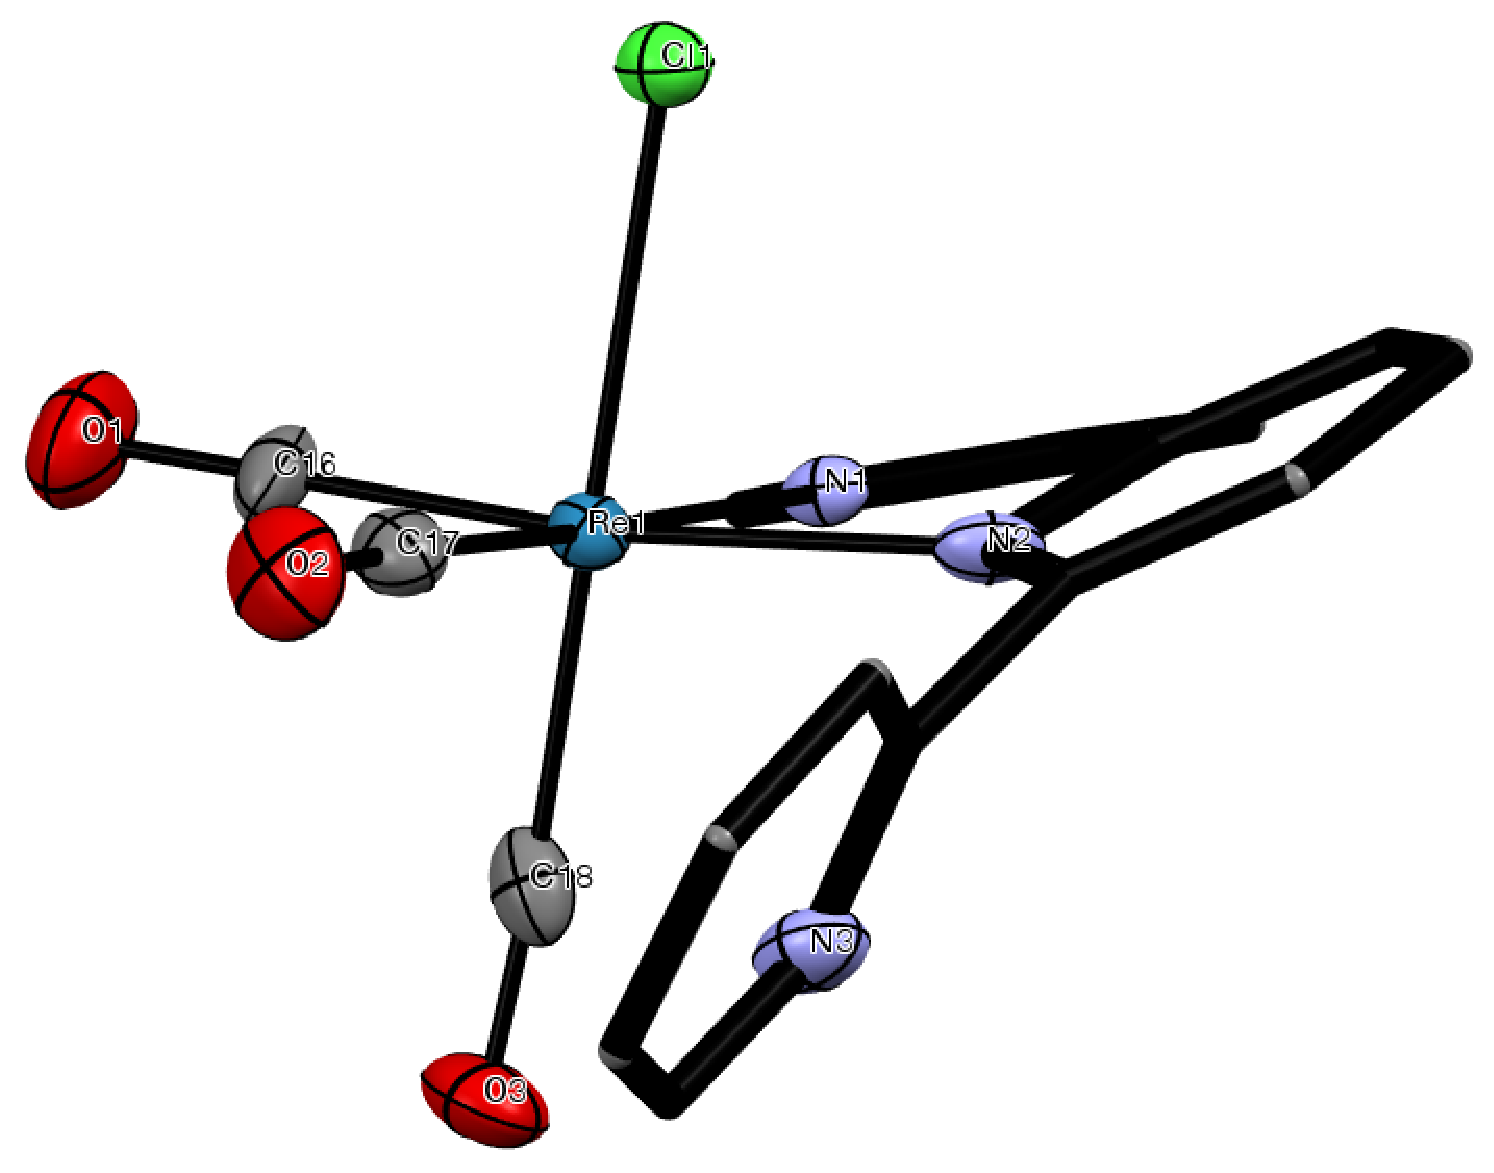
\includegraphics[clip=true, width=\textwidth, height=50mm, keepaspectratio]{images/xray1b.eps}
 \end{subfigure}
 \begin{subfigure}[b]{0.49\textwidth}
  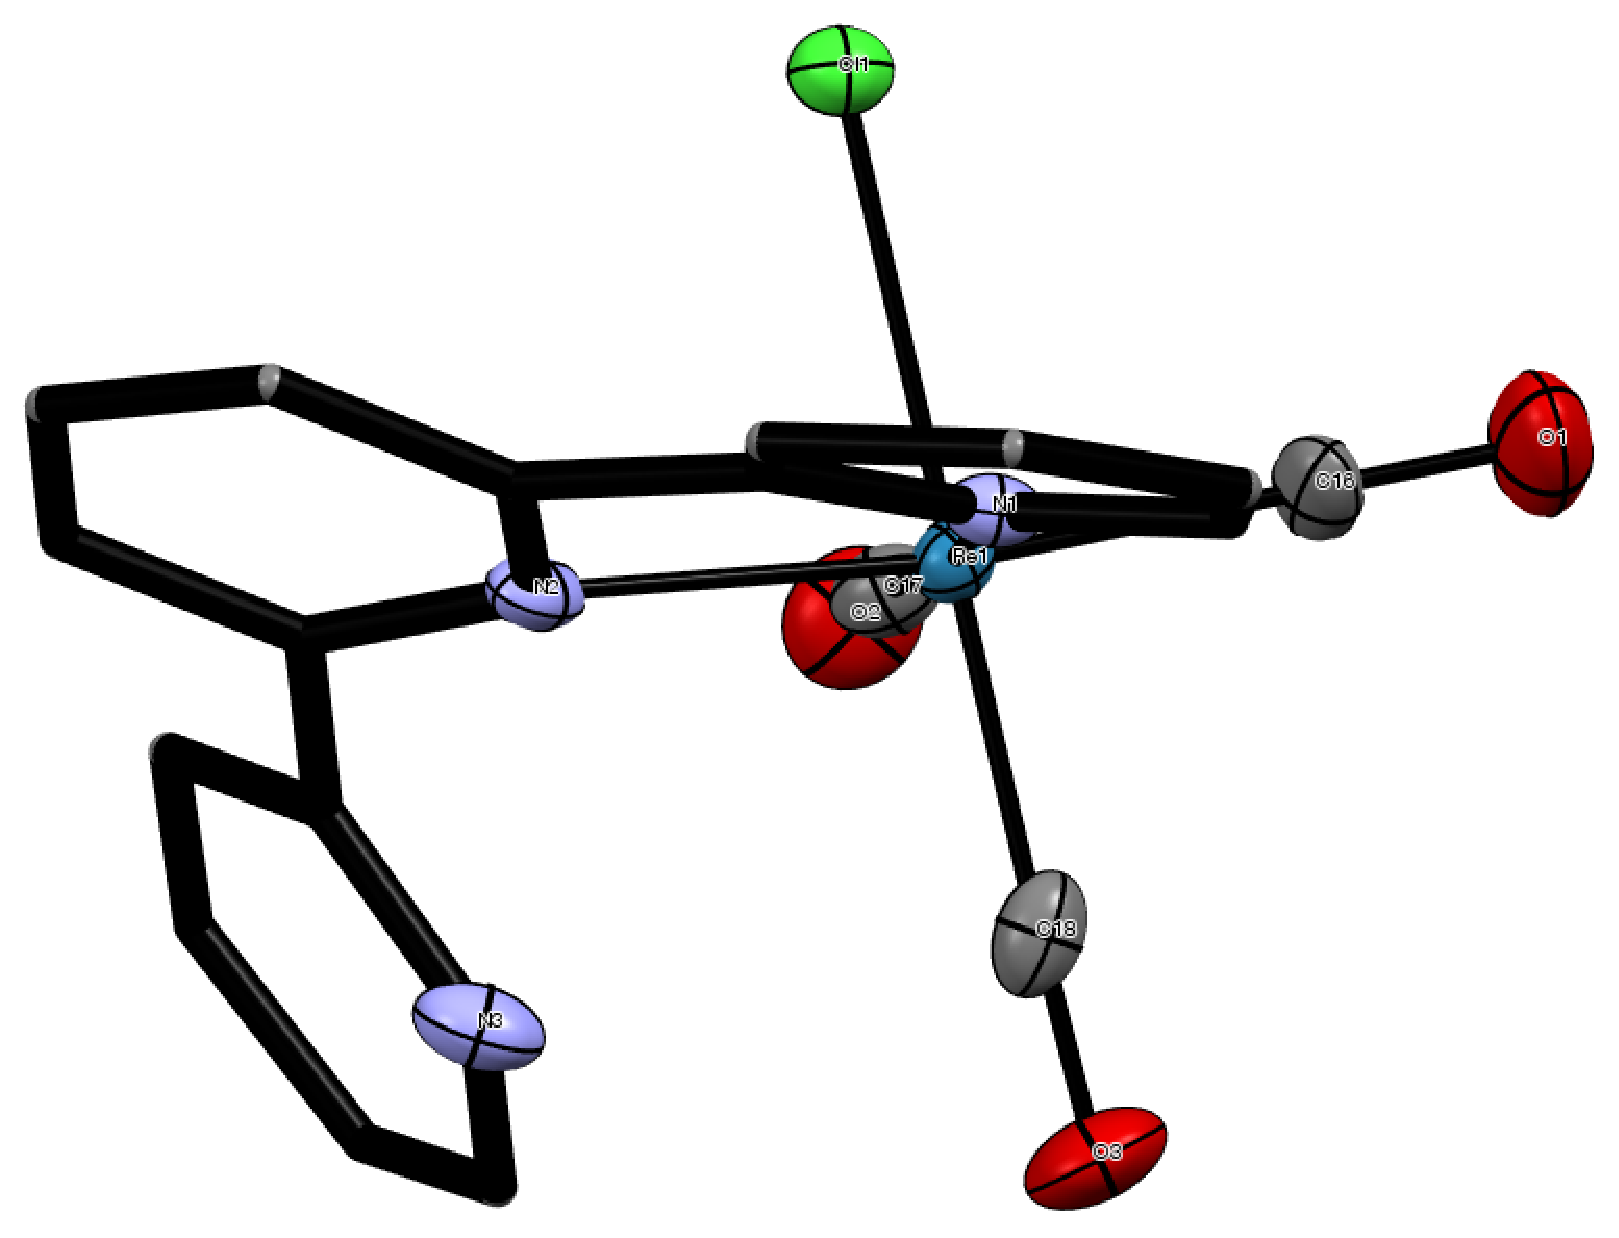
\includegraphics[clip=true, width=\textwidth, height=50mm, keepaspectratio]{images/xray1c.eps}
 \end{subfigure}
  \begin{subfigure}[b]{0.49\textwidth}
  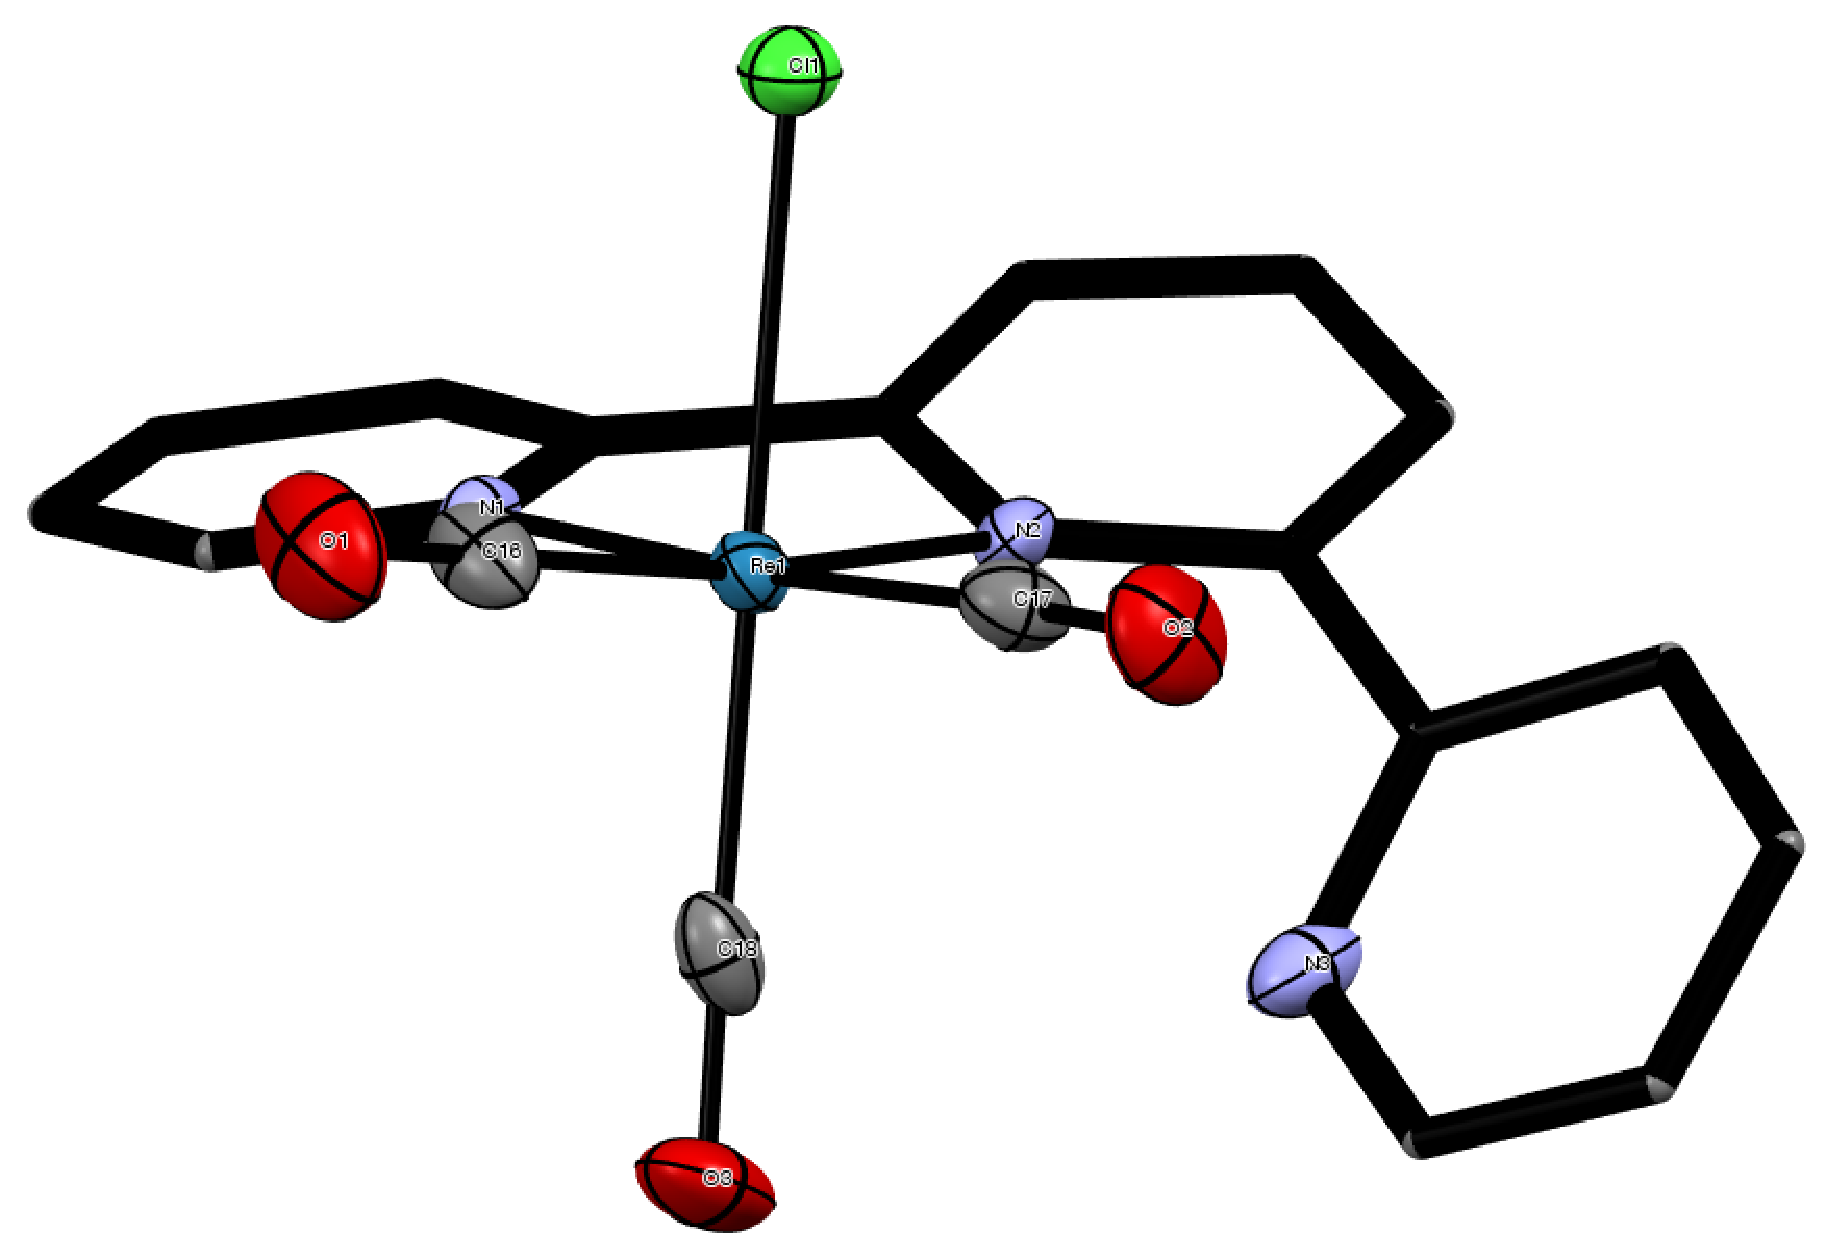
\includegraphics[clip=true, width=\textwidth, height=50mm, keepaspectratio]{images/xray1d.eps}
 \end{subfigure}
 \begin{subfigure}[b]{\textwidth}
  \centering
  \includegraphics[clip=true, width=\textwidth, height=75mm, keepaspectratio]{images/xray1uc.eps}
  \caption{Full unit cell representation of \textbf{2.1}}
 \end{subfigure}
\caption[X-ray crystal structure of \textbf{2.1}]{X-ray crystal structure of \textbf{2.1}. Co-crystallized chloroform, hydrogen atoms, and thermal ellipsoids of ligand carbon atoms are omitted for clarity.}
\label{fig.xray21}
\end{figure}

\begin{figure}[!ht]
 \centering
 \begin{subfigure}[b]{0.49\textwidth}
  \includegraphics[clip=true, width=\textwidth, height=50mm, keepaspectratio]{images/xray2a.eps}
 \end{subfigure}
 \begin{subfigure}[b]{0.49\textwidth}
  \includegraphics[clip=true, width=\textwidth, height=50mm, keepaspectratio]{images/xray2b.eps}
 \end{subfigure}
 \begin{subfigure}[b]{0.49\textwidth}
  \includegraphics[clip=true, width=\textwidth, height=50mm, keepaspectratio]{images/xray2c.eps}
 \end{subfigure}
 \begin{subfigure}[b]{\textwidth}
  \centering
  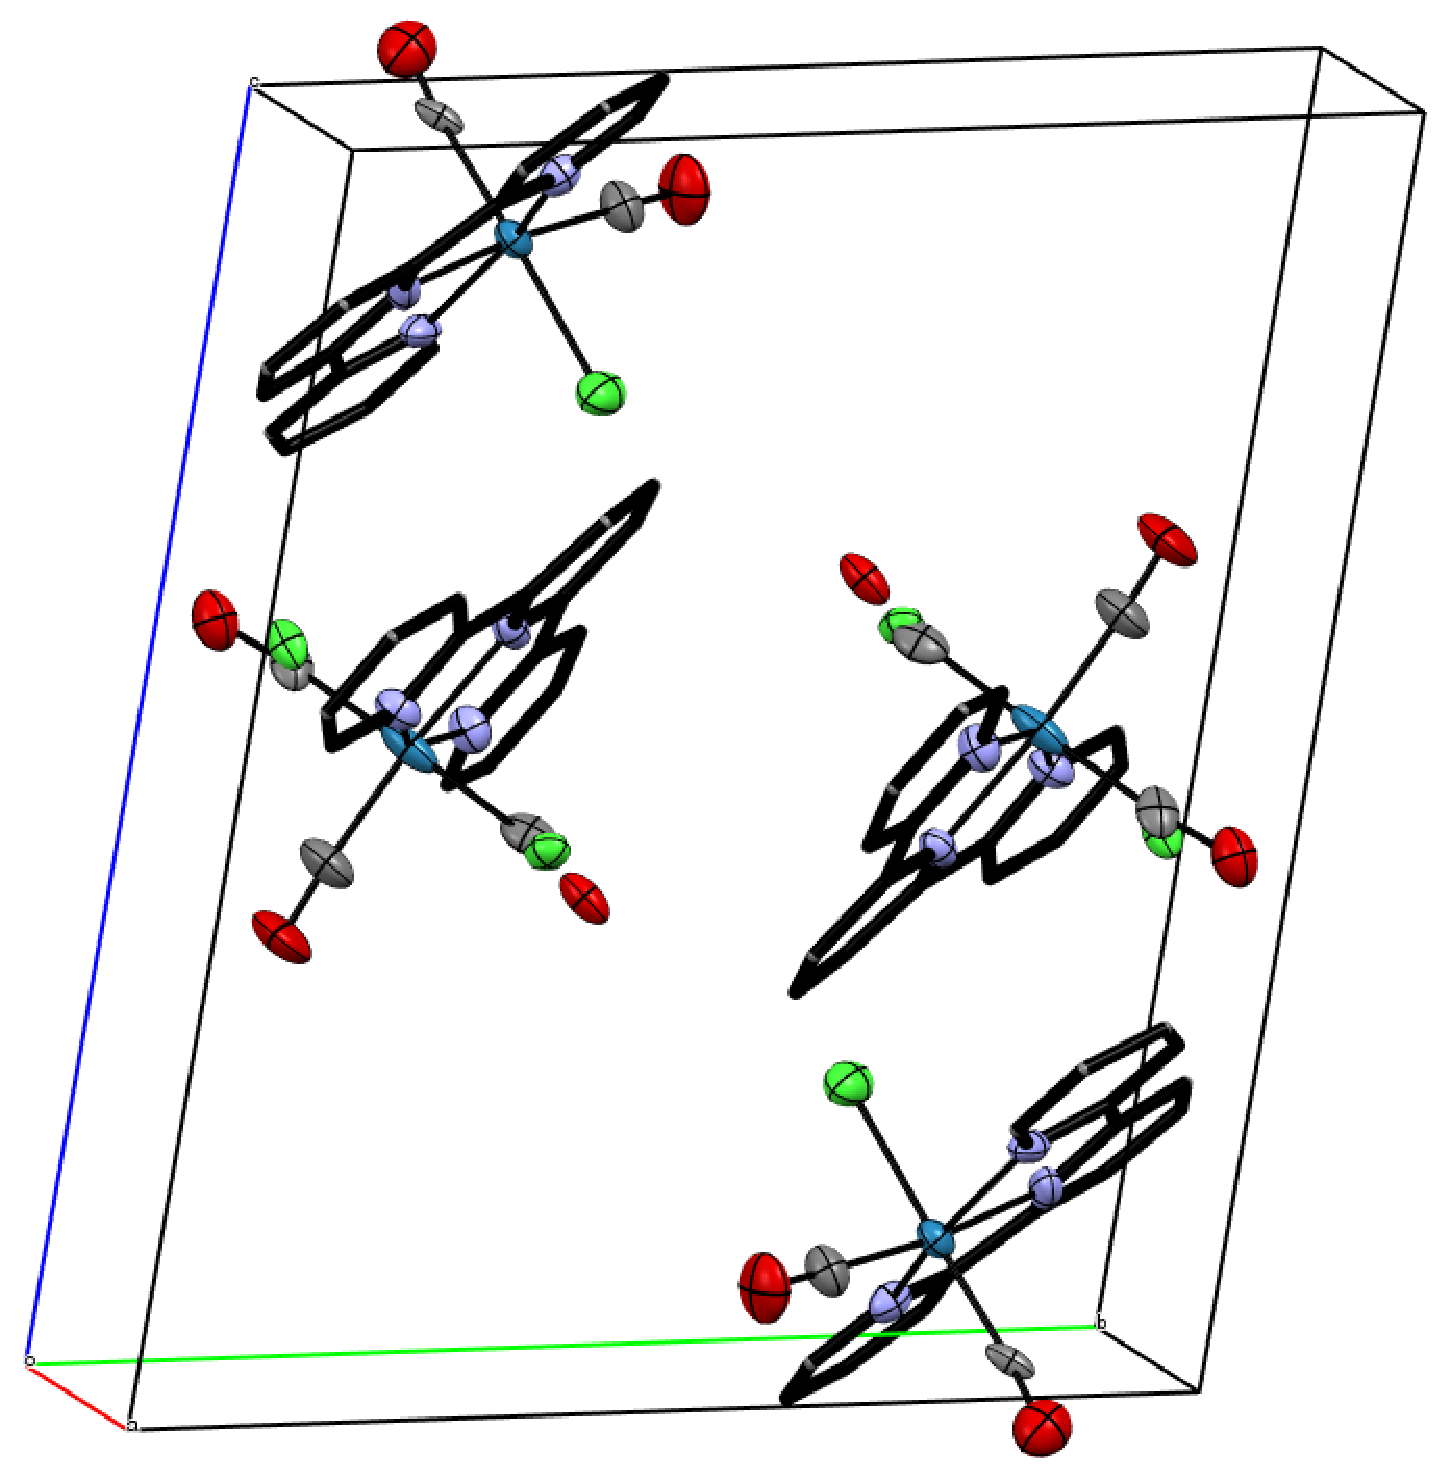
\includegraphics[clip=true, width=\textwidth, height=75mm, keepaspectratio]{images/xray2uc.eps}
  \caption{Full unit cell representation of \textbf{2.2}}
 \end{subfigure}
\caption[X-ray crystal structure of \textbf{2.2}]{X-ray crystal structure of \textbf{2.2}. Co-crystallized chloroform, hydrogen atoms, and thermal ellipsoids of ligand carbon atoms are omitted for clarity.}
\label{fig.xray22}
\end{figure}

\begin{figure}[!ht]
 \centering
 \begin{subfigure}[b]{0.49\textwidth}
  \includegraphics[clip=true, width=\textwidth, height=50mm, keepaspectratio]{images/xray3a.eps}
 \end{subfigure}
 \begin{subfigure}[b]{0.49\textwidth}
  \includegraphics[clip=true, width=\textwidth, height=50mm, keepaspectratio]{images/xray3b.eps}
 \end{subfigure}
 \begin{subfigure}[b]{0.49\textwidth}
  \includegraphics[clip=true, width=\textwidth, height=50mm, keepaspectratio]{images/xray3c.eps}
 \end{subfigure}
 \begin{subfigure}[b]{0.49\textwidth}
  \includegraphics[clip=true, width=\textwidth, height=50mm, keepaspectratio]{images/xray3d.eps}
 \end{subfigure}
 \begin{subfigure}[b]{\textwidth}
  \centering
  \includegraphics[clip=true, width=\textwidth, height=75mm, keepaspectratio]{images/xray3uc.eps}
  \caption{Full unit cell representation of \textbf{2.3}}
 \end{subfigure}
\caption[X-ray crystal structure of \textbf{2.3}]{X-ray crystal structure of \textbf{2.3}. Hydrogen atoms, and thermal ellipsoids of ligand carbon atoms are omitted for clarity.}
\label{fig.xray23}
\end{figure}

\begin{figure}[!ht]
 \centering
 \begin{subfigure}[b]{0.49\textwidth}
  \includegraphics[clip=true, width=\textwidth, height=50mm, keepaspectratio]{images/xray5a.eps}
 \end{subfigure}
 \begin{subfigure}[b]{0.49\textwidth}
  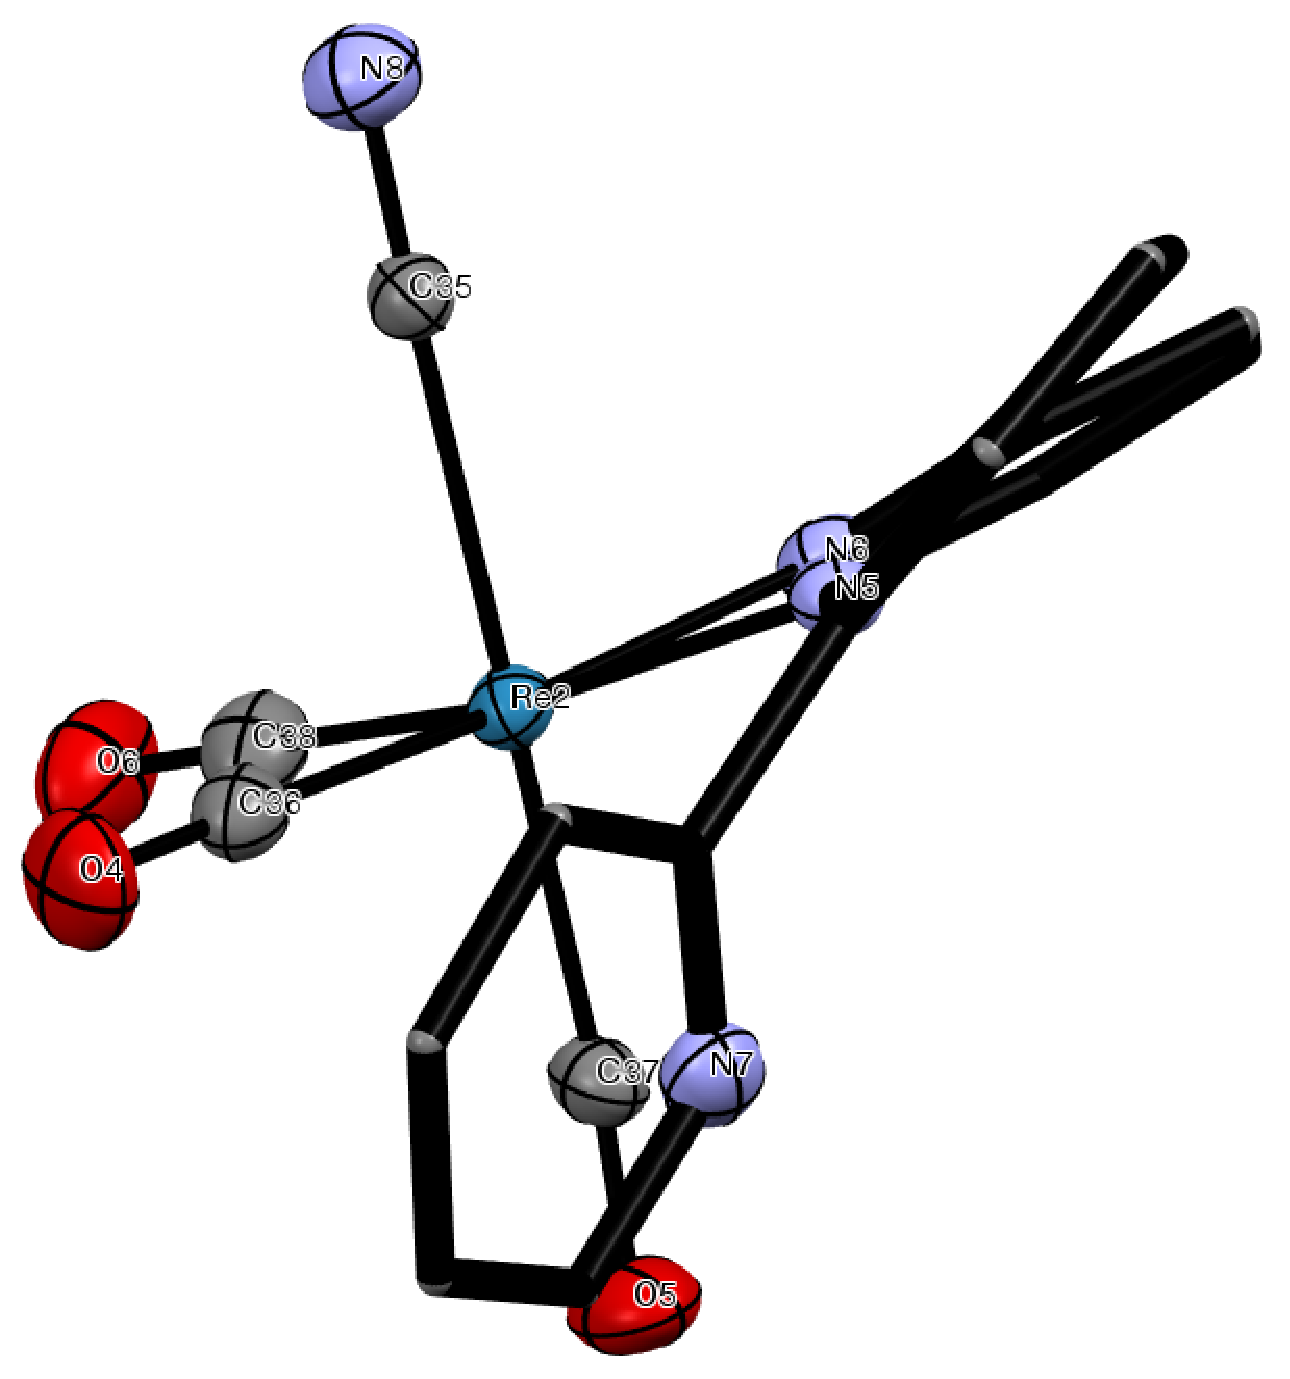
\includegraphics[clip=true, width=\textwidth, height=50mm, keepaspectratio]{images/xray5b.eps}
 \end{subfigure}
 \begin{subfigure}[b]{0.49\textwidth}
  \includegraphics[clip=true, width=\textwidth, height=50mm, keepaspectratio]{images/xray5c.eps}
 \end{subfigure}
 \begin{subfigure}[b]{0.49\textwidth}
  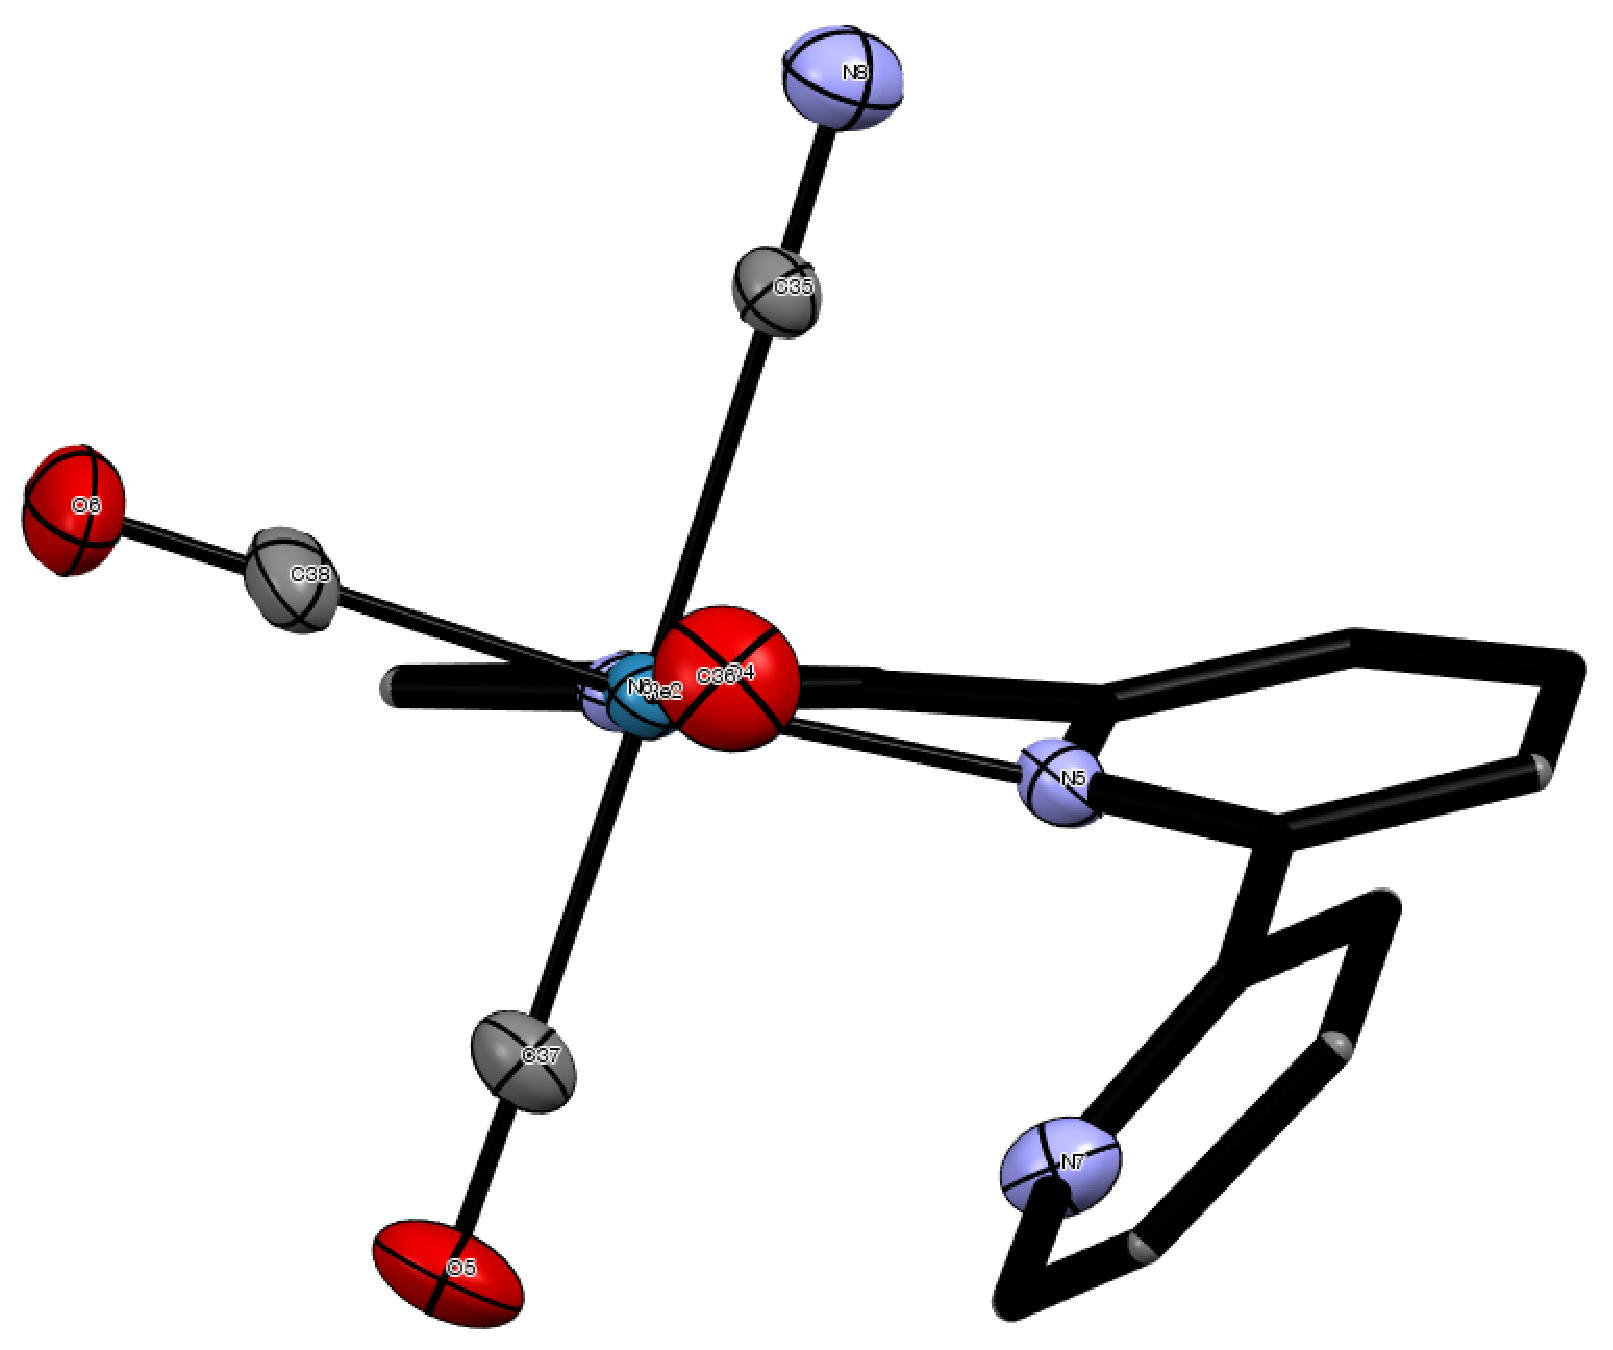
\includegraphics[clip=true, width=\textwidth, height=50mm, keepaspectratio]{images/xray5d.eps}
 \end{subfigure}
 \begin{subfigure}[b]{\textwidth}
  \centering
  \includegraphics[clip=true, width=\textwidth, height=75mm, keepaspectratio]{images/xray5uc.eps}
  \caption{Full unit cell representation of \textbf{2.5}}
 \end{subfigure}
\caption[X-ray crystal structure of \textbf{2.5}]{X-ray crystal structure of \textbf{2.5}. Hydrogen atoms, and thermal ellipsoids of ligand carbon atoms are omitted for clarity.}
\label{fig.xray25}
\end{figure}

\begin{figure}[!ht]
 \centering
 \begin{subfigure}[b]{0.49\textwidth}
  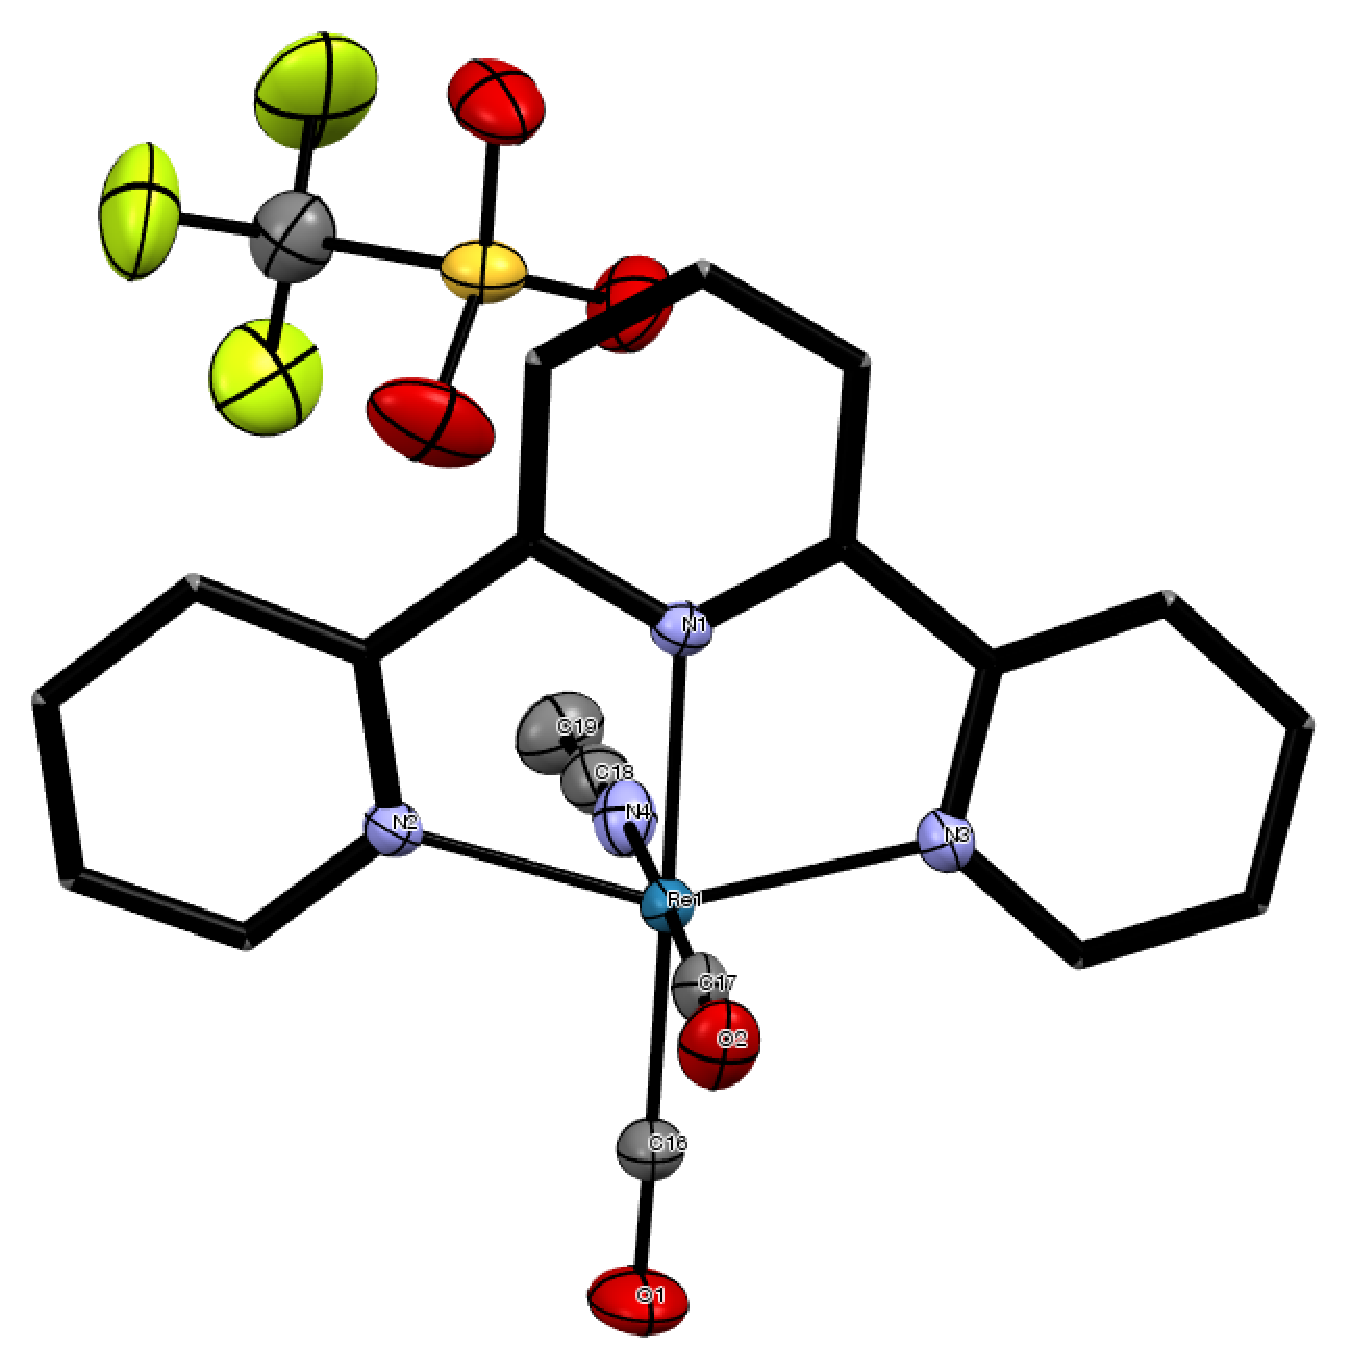
\includegraphics[clip=true, width=\textwidth, height=50mm, keepaspectratio]{images/xray8a.eps}
 \end{subfigure}
 \begin{subfigure}[b]{0.49\textwidth}
  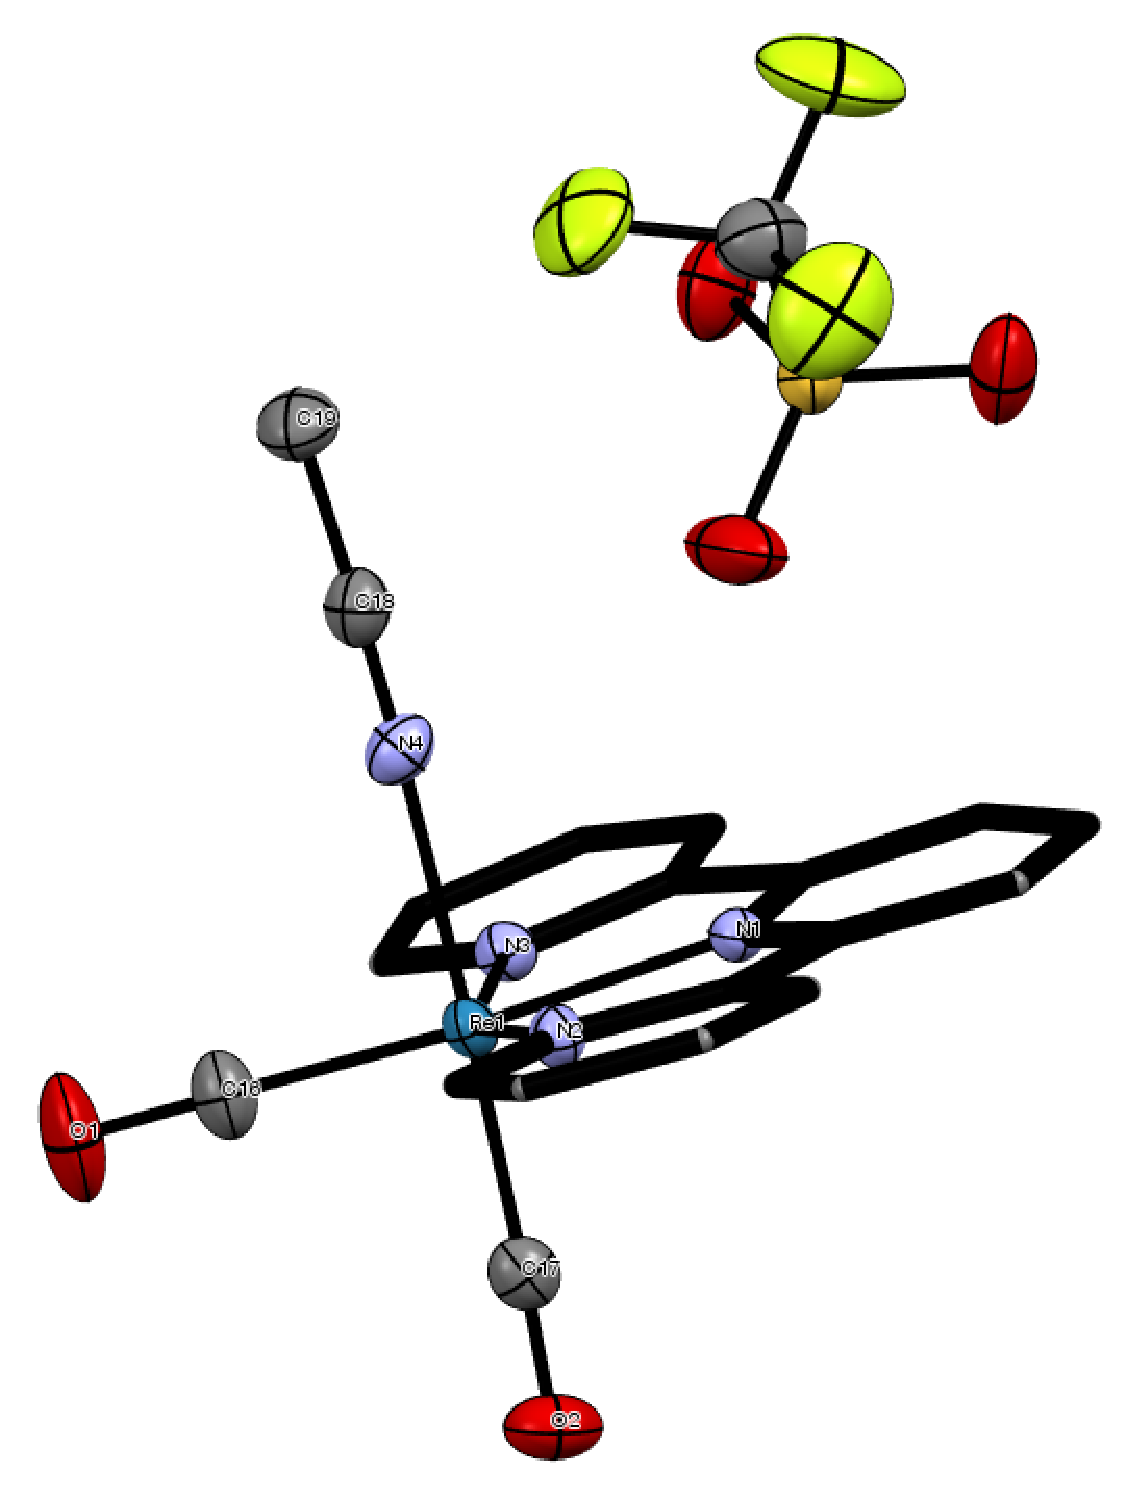
\includegraphics[clip=true, width=\textwidth, height=50mm, keepaspectratio]{images/xray8b.eps}
 \end{subfigure}
 \begin{subfigure}[b]{0.49\textwidth}
  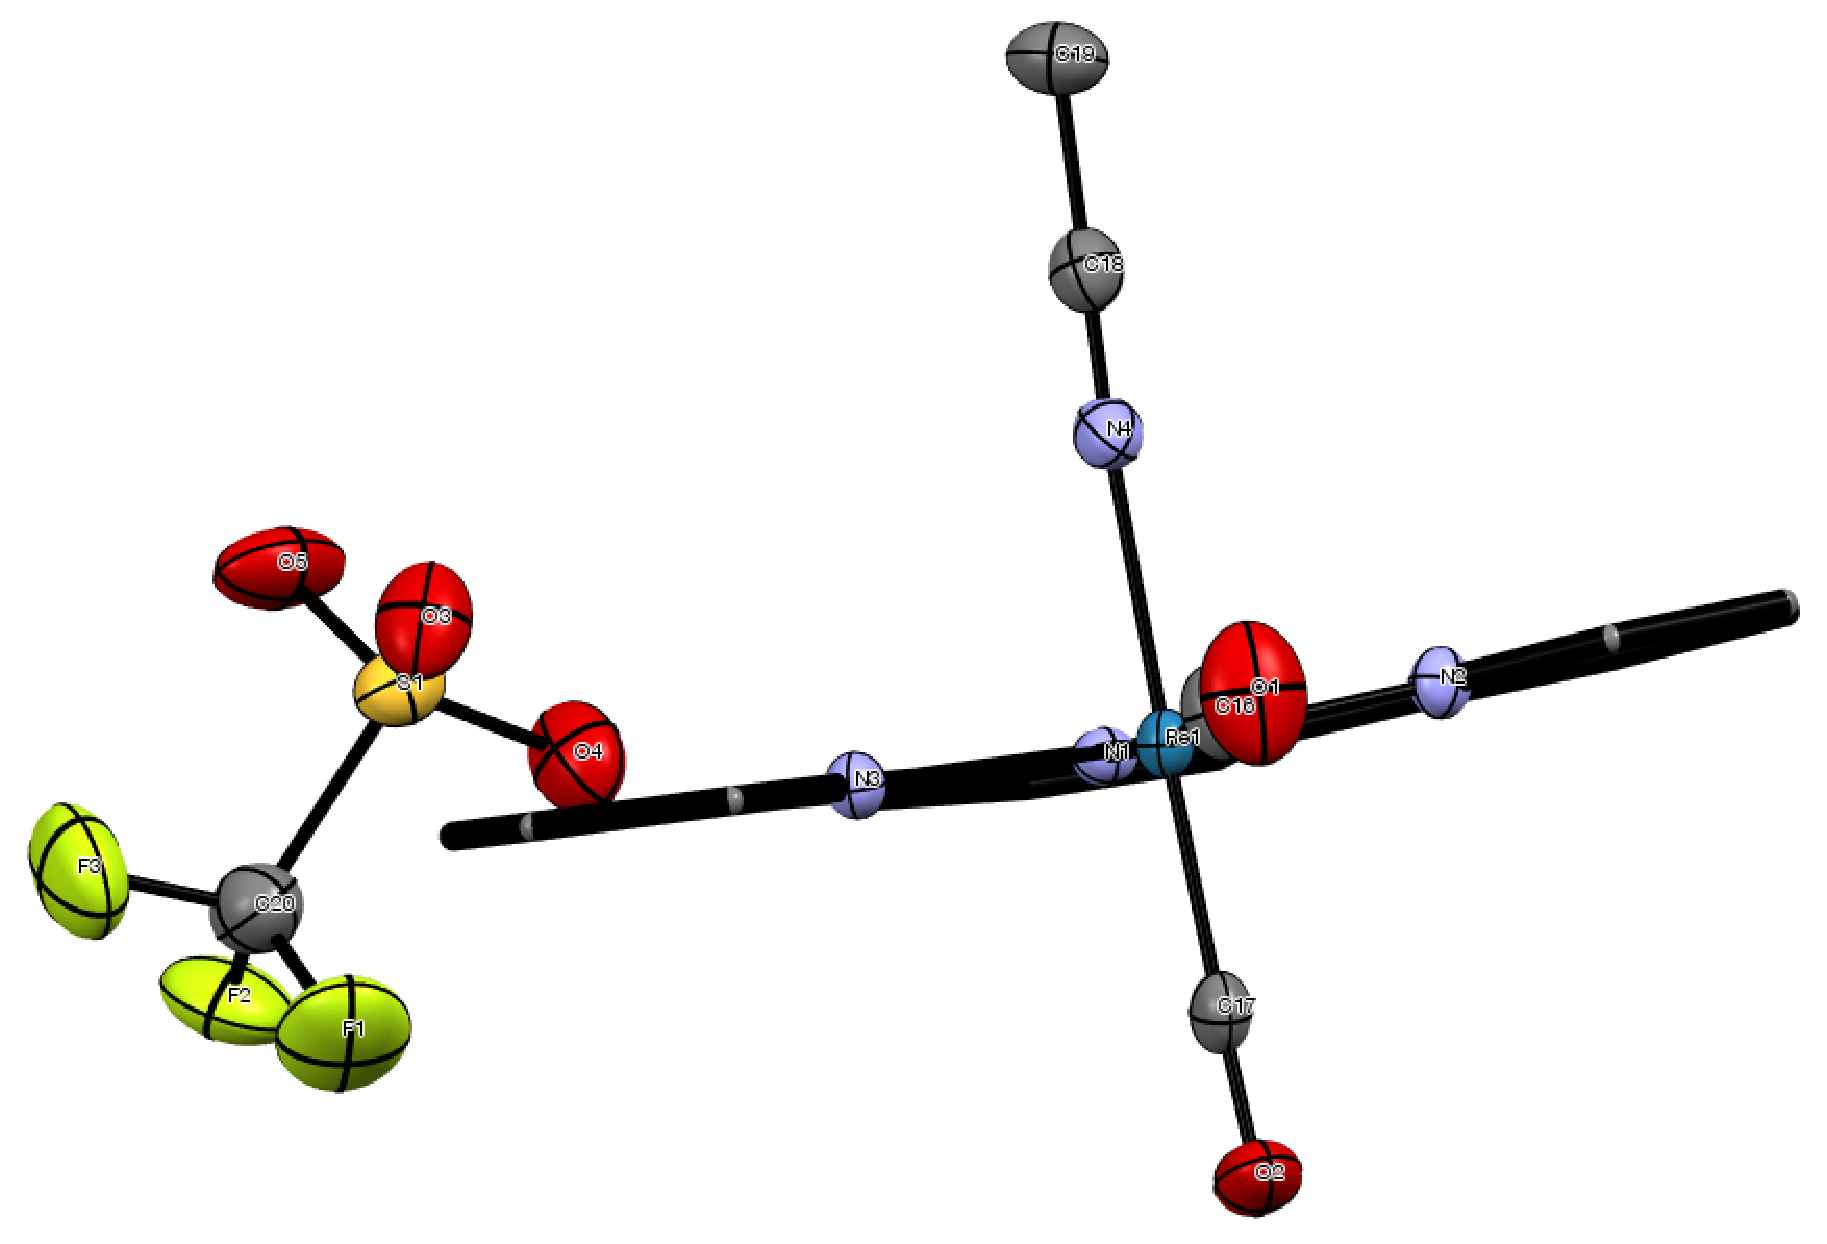
\includegraphics[clip=true, width=\textwidth, height=50mm, keepaspectratio]{images/xray8c.eps}
 \end{subfigure}
 \begin{subfigure}[b]{0.49\textwidth}
  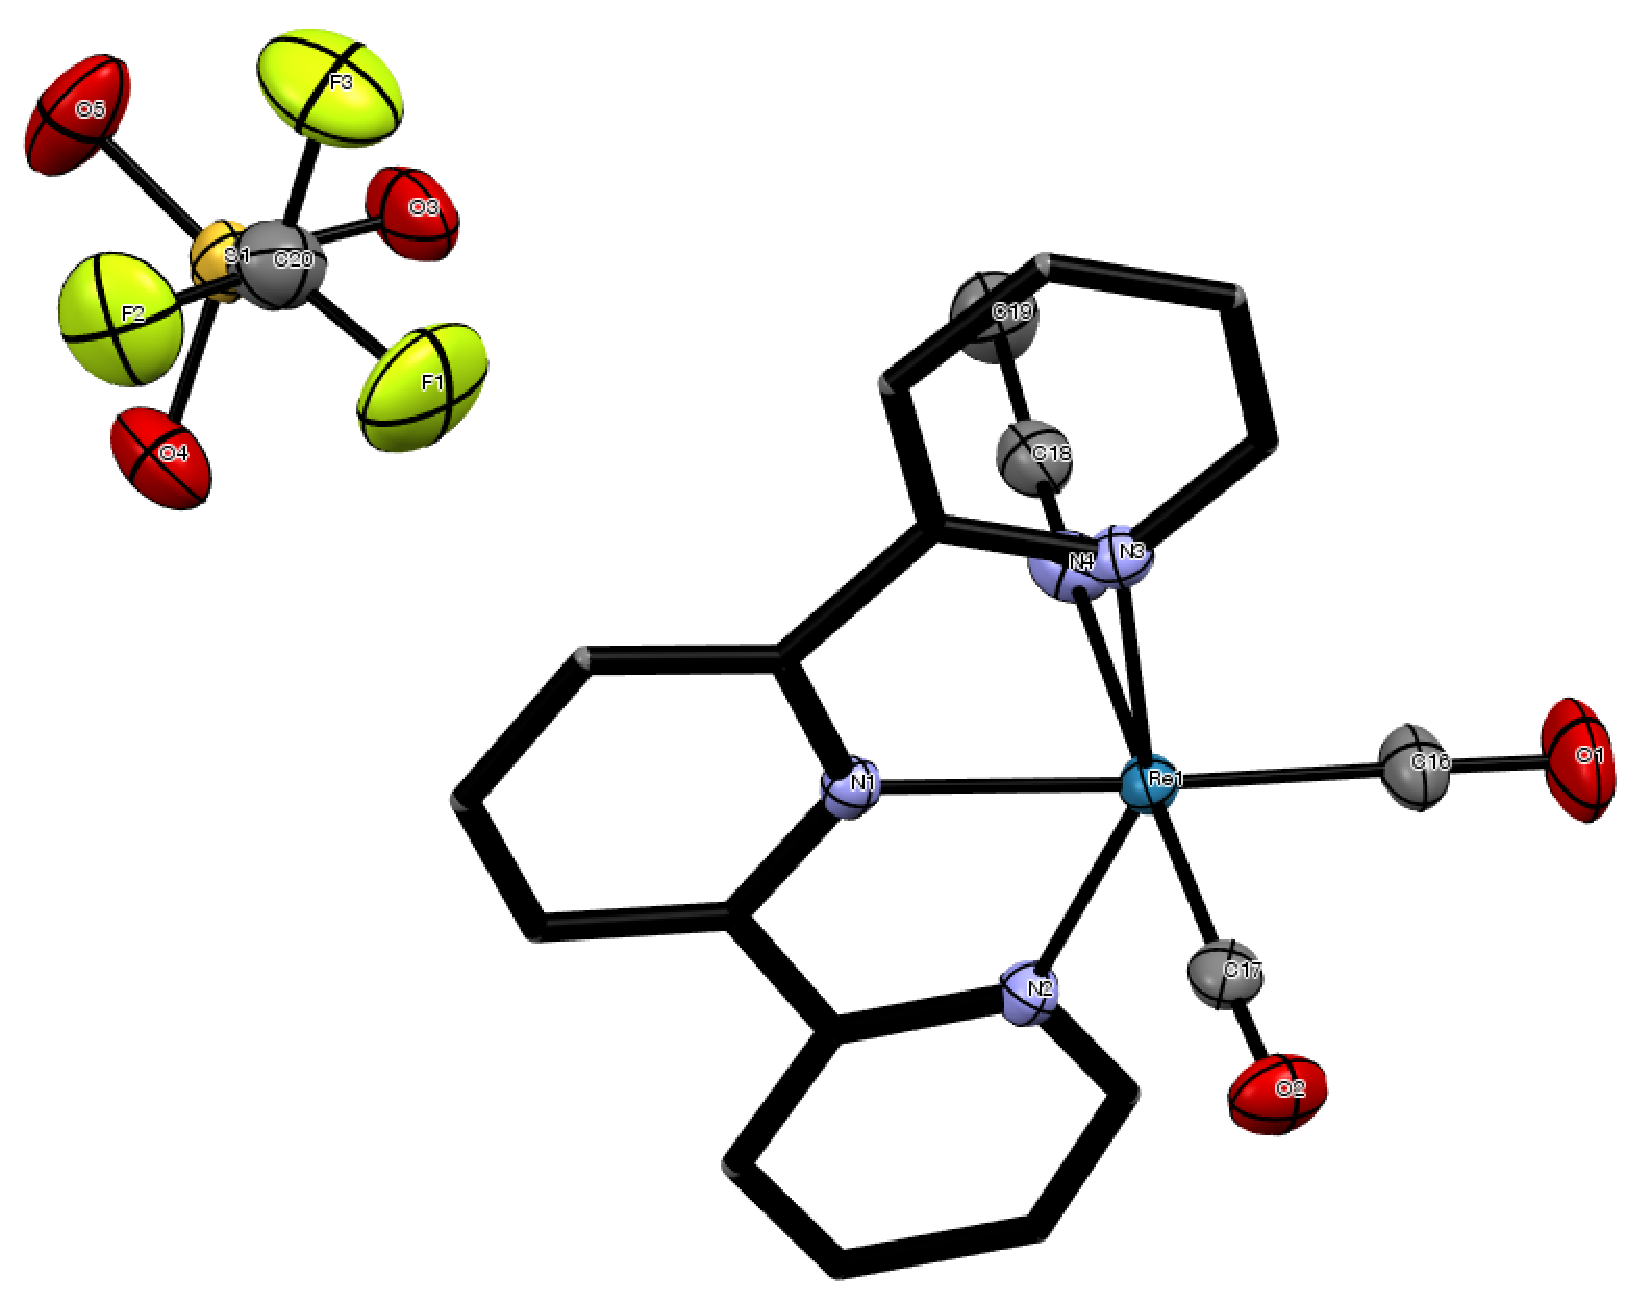
\includegraphics[clip=true, width=\textwidth, height=50mm, keepaspectratio]{images/xray8d.eps}
 \end{subfigure}
 \begin{subfigure}[b]{\textwidth}
  \centering
  \includegraphics[clip=true, width=\textwidth, height=75mm, keepaspectratio]{images/xray8uc.eps}
  \caption{Full unit cell representation of \textbf{2.8}}
 \end{subfigure}
\caption[X-ray crystal structure of \textbf{2.8}]{X-ray crystal structure of \textbf{2.8}. Hydrogen atoms, and thermal ellipsoids of ligand carbon atoms are omitted for clarity.}
\label{fig.xray28}
\end{figure}

\section{(terpy-$\kappa^2$-N,N$^\prime$)\ce{Re(CO)3Cl} (2.1)}\label{sec.c1}
\ce{Re(CO)5Cl} (201~mg,  0.556~mmol) and 2,2’:6’,2’’ terpyridine (129~mg, 0.553~mmol) were mixed in 60~mL of toluene. The reaction mixture was heated to 100°C for 1 hour under N2. During this time the solution turned a bright red. Upon cooling a yellow precipitate was formed. The solution was filtered, and the solid was washed with diethyl ether, and dried under vacuum. Compound \textbf{1} is a bright yellow powder that was isolated in 70~\% yield (208~mg). Crystals were obtained from chloroform with addition of a small amount of hexanes as counter solvent. TGA: 8~\% mass loss from 240-280~$^\circ$C.  FTIR: 2019, 1981, 1889 cm\ce{^{-1}} (\textit{v} C=O). \ce{^1H} NMR (\ce{CD3CN}, 400 MHz): $\delta$ 9.06 (ddd, J=5.6, 1.7, 0.8 Hz, 1H), 8.77 (ddd, J=4.9 Hz, 1H), 8.49 (td, J=8.2, 1.5 Hz, 2H), 8.28 (t, J=7.9 Hz, 1H), 8.22 (td, J=8.1, 1.6 Hz, 1H), 7.96 (td, J=7.8, 1.8 Hz, 1H), 7.79 (dt, J=7.8, 1.1 Hz, 1H), 7.80 (dd, J=7.7, 1.0 Hz, 1H), 7.63 (ddd, J=7.6, 5.5, 1.2 Hz, 1H), 7.55 (ddd, J=7.6, 5.0, 1.0 Hz, 1H). Elemental analysis calculated (\%) for [\ce{C18H11ReClN3O3}]: C 40.11, H 2.06, N 7.80, found C 39.96, H 2.09, N 7.69.

\section{(terpy-$\kappa^3$-N,N$^\prime$,N$^{\prime \prime}$)\ce{Re(CO)2Cl} (2.2)}\label{sec.c2}
Compound \textbf{1} (101~mg, 0.187~mmol) was placed in a tube furnace and heated to 240~$^\circ$C under \ce{N2} flow for 60 minutes. A black solid was collected (90~mg) at 94~\% yield based on the formula for \textbf{2}. Crystals were obtained from chloroform with addition of a small amount of hexanes as counter solvent. FTIR: 1872, 1788 cm\ce{^{-1}} (\textit{v} C=O). \ce{^1H} NMR (\ce{CD3CN}, 400 MHz): $\delta$ 8.70 (ddd, J=4.7, 1.8, 0.9 Hz, 2H), 8.65 (dt, J=8.0, 1.0, 1.0, 2H), 8.47 (d, J=7.8 Hz, 2H), 8.03 (t, J=7.8 Hz, 1H), 7.95 (td, J=7.7, 7.7, 1.9 Hz, 2H), 7.43 (ddd, J=7.5, 4.8, 1.2 Hz, 2H). Elemental analysis calculated (\%) for [\ce{C17H11ReClN3O2}]: C~39.96, H~2.17, N~8.22, found C~39.62, H~2.09, N~7.99.

\section{(terpy-$\kappa^2$-N,N$^\prime$)\ce{Re(CO)3Br} (2.3)}\label{sec.c3}
\ce{Re(CO)5Br} (191~mg, 470~mmol) and 2,2’:6’2’’ terpyridine (129~mg, 0.553~mmol) were allowed to react under conditions analogous to the preparation of \textbf{1}. A bright yellow powder was obtained, 0.223 g (0.382~mmol, 81~\%). FTIR: 2012, 1910, 1886 cm\ce{^{-1}} (\textit{v} C=O). \ce{^1H} NMR (\ce{CD3CN}, 400 MHz): $\delta$ 9.07 (ddd, J=5.6, 1.6, 0.9 Hz, 1H), 8.77 (ddd, J=4.6, 1.5, 0.8 Hz, 1H), 8.52 – 8.48 (m, 2H), 8.28 (t, J=7.9 Hz, 1H), 8.21 (td, J=8.0, 1.6 Hz, 1H), 7.97 (td, J=7.8, 1.8 Hz, 1H), 7.80 – 7.75(m, 2H), 7.63 (ddd, J=7.6, 5.5, 1.2 Hz, 1H), 7.55 (ddd, J=7.7, 4.9, 1.1 Hz, 1H). Elemental analysis calculated (\%) for [\ce{C18H11ReBrN3O3}]: C~37.06, H~1.90, N~7.20, found C~36.94, H~1.92, N~7.00.  

\section{(terpy-$\kappa^3$-N,N$^\prime$,N$^{\prime \prime}$)\ce{Re(CO)2Br} (2.4)}\label{sec.c4}
Compound \textbf{3} (182~mg, 0.312~mmol) was placed in an tube furnace and heated to 230~$^\circ$C under \ce{N2} flow for 60 minutes. A black solid was collected, 0.155~mg (0.279~mmol, 89~\% yield). Crystals were obtained from chloroform with addition of a small amount of hexanes as counter solvent. FTIR: 1873, 1794 cm\ce{^{-1}} (\textit{v} C=O). \ce{^1H} NMR (\ce{CD3CN}, 400 MHz): $\delta$ 8.95 (d, J=5.4 Hz, 2H), 8.24 (t, J = 8.1Hz, 4H), 8.05 (dd, J=8.2, 7.7 Hz, 1H), 7.90(td, J=7.9, 1.7 Hz, 2H), 7.63 (ddd, J=7.3, 5.5, 1.2 Hz, 2H). Elemental analysis calculated (\%) for [\ce{C17H11ReBrN3O2}]: C~36.76, H~2.00, N~7.57, found C~36.66, H~2.00, N~7.50.

\section{(terpy-$\kappa^2$-N,N$^\prime$)\ce{Re(CO)3CN} (3)} \label{sec.c5}
To \textbf{1} (80~mg, 0.148~mmol), \ce{AgCF3SO3} (46~mg, 0.179~mmol) was added in 10~mL \ce{CH2Cl2}. The reaction was stirred 18~h and kept dark under \ce{N2} atmosphere. Solution was filtered to remove salts, then reduced in volume. Cold diethyl ether was used to precipitate product. Yellow-grey powder (\textbf{7a}) was collected by filtration, yielding 38mg (40~\%). Crystals were grown from saturated chloroform with hexanes as countersolvent for X-ray crystallography. FTIR: 2013, 1905, 1884 cm\ce{^{-1}} (\textit{v} C=O). \ce{^1H} NMR (\ce{CD3CN}, 400 MHz): $\delta$ 9.08 (dd, J=5.40, 0.49 Hz, 1 H), 8.78 (dd, J=5.10, 0.59 Hz, 1 H), 8.53 (dd, J=8.18, 0.93 Hz, 1 H), 8.50 (d, J=8.23 Hz, 1 H), 8.30 (t, J=7.90 Hz, 1 H), 8.23 (td, J=7.94, 1.57 Hz, 2 H), 7.98 (td, J=7.76, 1.71 Hz, 1 H), 7.80 (dd, J=7.79, 1.03 Hz, 1 H), 7.77 (d, J=7.74 Hz, 0 H), 7.64 (ddd, J=7.50, 5.50, 1.08 Hz, 1 H), 7.55 (ddd, J=7.62, 4.92, 0.98 Hz, 2 H).  Elemental analysis calculated (\%) for [\ce{C19H11N4O3Re}]: C~43.10, H~2.09, N~10.58, found C~40.06, H~2.06, N~9.85.

\section{(terpy-$\kappa^3$-N,N$^\prime$,N$^{\prime \prime}$)\ce{Re(CO)2CN} (2.6)} \label{sec.c6}
To \textbf{2} (77~mg,  0.143~mmol), \ce{AgSO3CF3} (47~mg,  0.183~mmol) was added in 15~mL \ce{CH2Cl2}. Solution was stirred for 18~h in the dark under \ce{N2} atmosphere. Solution was filtered, then reduced to minimal volume. Cold diethyl ether was added dropwise to precipitate product. Collected by filtration and washed with additional cold ether, yielding 75~mg (120~mmol, 80~\%).  Crystals grown from saturated methylene chloride, with hexanes as countersolvent for x-ray crystallography. \ce{^1H} NMR (\ce{CD3CN}, 400 MHz): $\delta$ 8.60(ddt, J=4.8, 1.7, 0.8, 0.8 Hz, 2H), 8.48 (dq, J=8.0, 1.0 Hz, 2H), 8.37 (dd, J=7.9, 0.8 Hz, 2H), 8.07 (dd, J=8.0, 7.6 Hz, 1 H), 7.94 (ddd, J=7.9, 7.5, 1.8 Hz, 2H) 7.43 (ddd J=7.4, 4.8, 1.2 Hz, 2H). Elemental analysis calculated (\%) for [\ce{C18H11N4O2Re}]: C~43.11, H~2.21, N~11.17, found C~40.26, H~2.67, N~9.60.

\todo{CN Experimental, masses, \sout{ir}, \sout{nmr},  \sout{EA}}

\section{(terpy-$\kappa^2$-N,N$^\prime$)\ce{Re(CO)3OTf} (2.7)}\label{sec.c7}
To \textbf{1} (80~mg, 0.148~mmol), \ce{AgCF3SO3} (46~mg, 0.179~mmol) was added in 10~mL \ce{CH3CN}. The reaction was stirred 18~h and kept dark. Solution was filtered to remove salts, then reduced in volume. Cold diethyl ether was used to precipitate product. Yellow-grey powder (\textbf{7a}) was collected by filtration, yielding 38~mg (40~\%). Crystals were grown from saturated chloroform with hexanes as countersolvent for X-ray crystallography. FTIR: 2030, 1895, 1890 cm\ce{^{-1}} (\textit{v} C=O), 1280, 1228, 1204 cm\ce{^{-1}} (\textit{v} \ce{SO3}). \ce{^1H} NMR (\ce{CD3CN}, 400 MHz): $\delta$ 9.05 (ddd, J=5.5, 1.6, 0.8 Hz, 1H), 8.79 (ddd, J=4.9, 1.8, 1.1 Hz, 1H), 8.57 (dd, J=8.1, 0.9 Hz, 1H), 8.54 (dt, J=8.2, 1.1 Hz, 1H), 8.37 (t, J=7.9 Hz, 1H), 8.31 (td, J=8.0, 1.6 Hz, 1H), 8.03 (td, J=7.7, 1.7 Hz, 1H), 7.87 (dd, J=7.8, 1.0 Hz, 1H), 7.75 (dt, J=7.8, 1.1 Hz, 1H), 7.72 (ddd, J=7.4, 5.9, 1.1 Hz, 1H), 7.61 (ddt, J=7.7, 4.8, 0.5, 0.5 Hz, 1H).  Elemental analysis calculated (\%) for [\ce{C19H11ReN3O6F3S}]: C~34.97, H~1.70, N~6.44, found C~31.80, H~1.73, N~5.33.

Alternately, to \textbf{1} (72~mg, 0.134~mmol) was added 10~mL \ce{CF3SO3H} (excess) and temperature was increased to 100~$^\circ$C for 20 minutes. A black solution was neutralized with addition of 5\% \ce{Na2CO3} in \ce{H2O}. Product was extracted with \ce{CHCl3}, then dried under vacuum to yield a brown solid (\textbf{7b}) (47~mg, 54~\%).

\section{(terpy-$\kappa^3$-N,N$^\prime$,N$^{\prime \prime}$)\ce{Re(CO)2OTf} (2.8)}\label{sec.c8}
To \textbf{2} (77~mg,  0.143~mmol), \ce{AgSO3CF3} (47~mg,  0.183~mmol) was added in 15~mL \ce{CH3CN}. Solution was refluxed for 6~h in the dark under \ce{N2} atmosphere. Solution was filtered, then reduced to minimal volume. Cold diethyl ether was added dropwise to precipitate product. Collected by filtration and washed with additional cold ether, yielding 75~mg (120~mmol, 80~\%).  Crystals grown from saturated methylene chloride, with hexanes as countersolvent for x-ray crystallography. FTIR: 1910, 1829 cm\ce{^{-1}} (\textit{v} C=O), 1259, 1224, 1143 cm\ce{^{-1}} (\textit{v} \ce{SO3}). \ce{^1H} NMR (\ce{CD3CN}, 400 MHz): $\delta$ 8.91(ddd, J=5.6, 1.6, 0.7 Hz, 2H), 8.32 (d, J=8.0 Hz, 2H), 8.28 (ddd, J=8.1, 1.4, 0.8 Hz, 2H), 8.19 (dd, J=8.8, 7.4 Hz, 1H), 8.02 (td, J=7.9, 1.5 Hz, 2H) 7.46 (ddd J=7.6, 5.6, 1.3 Hz, 2H).  Elemental analysis calculated (\%) for [\ce{C18H11ReF3SN3O5}]: C~34.62, H~1.78, N~6.37, found C~31.02, H~1.82, N~7.11.


